This Section is divided into two subsections. First we present the results of manual experiments that we evaluate by hand via the UI that we implemented in Section \ref{sec:manualver}.
The second Section \ref{sec:autover} contains results we obtained and evaluated automatically by running the simulations headlessly.

\subsection{Manual Verifications}
\label{sec:manualver}
insert here text we wrote on google docs on meeting day


\subsection{Automatic Verifications}
\label{sec:autover}
For the automatic evaluation we tried varying settings and ran them across all maps. Because the amount of different parameters and the hence large amount of graphs to interpret we will here only mention and display the settings that we deemed relevant information. To be statistically relevant every experiment setting is run 50 times and we then take the mean value of that for the graph. We also always include Towers in the maps.

Regarding the settings when we talk about normal settings, then these are the settings we found to work best using the manual mode. This consist of a spawn-amount of 14, a decay-threshold of -0.007 and a pheromone-increase threshold of 0.01.

First of we will start out by excluding the continuous vapour in the future Figures because as Figure \ref{fig:mirrorvaptick} clearly shows, the runtime is much larger than for all other three behaviours for the mirrored map. This behaviour was visible across all maps and settings, another example that stresses the uselessness of the continuous vapour is the runtime graph portrayed in Figure \ref{fig:shortlongvaptick} for the short and long map, the very basic map that all of them should be able to easily master.

\begin{figure}[H]
  \centering
  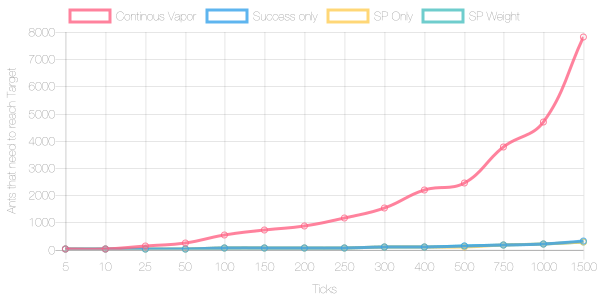
\includegraphics[width=1\linewidth]{images/normalmirroredwithtower-ticks-line}
  \caption{Comparing required Tick-Amount on the y-Axis to the target amount of ants to reach the target on the x-Axis for the mirrored map with normal settings.}
  \label{fig:mirrorvaptick}
\end{figure}

\begin{figure}[H]
  \centering
  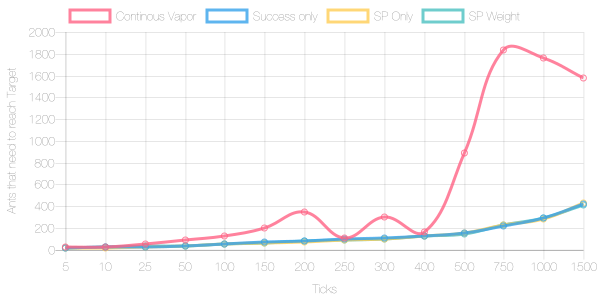
\includegraphics[width=1\linewidth]{images/normalshortandlongwithtowers-ticks-line}
  \caption{Comparing required Tick-Amount on the y-Axis to the target amount of ants to reach the target on the x-Axis for the short and long map with normal settings}
  \label{fig:shortlongvaptick}
\end{figure}

With the automatic evaluation we also further prove, that deducing pheromones upon death is rather counter-productive than helpful as visible in Figure \ref{fig:deathsubshitty}. But it does make sense given that any street-part an ant crossed on it's way to death will be deduced in pheromone. That means even a correct path like in the short and long map the longer one can lead to pheromone deduction and hence make the path unattractive again and future ants more likely to walk the even more dangerous path with more deaths.
Also for the weighted shortest path leaving death-substraction out even slightly improves the result. As for the non continuous vapor behaviour, not only does substraction not matter as much, but also all three perform quite similar.


\begin{figure}[H]
  \centering
  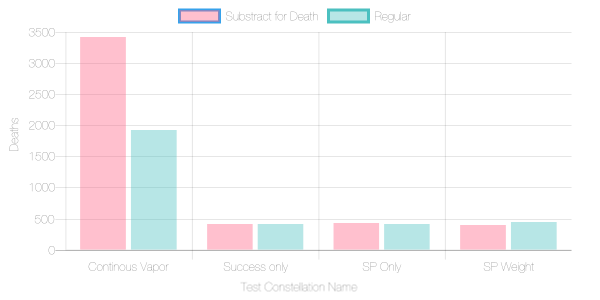
\includegraphics[width=1\linewidth]{images/normalshortandlongwithtowers-deaths}
  \caption{Comparing deaths for the different ant behaviours with and without substracting pheromones upon death on the short and long map with normal settings}
  \label{fig:deathsubshitty}
\end{figure}

The following graph, depicted in Figure \ref{fig:threesame} which doesn't include the continuous vapour any more shows, shows that the remaining three behaviours perform similar not only regarding death amount but also regarding their runtime.

\begin{figure}[H]
  \centering
  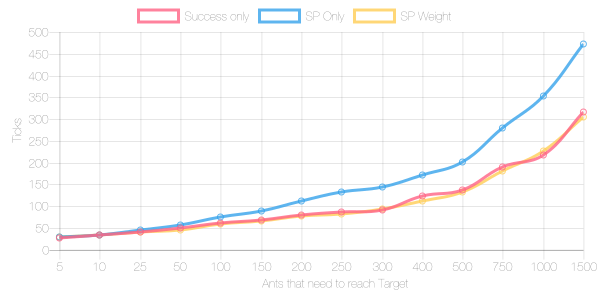
\includegraphics[width=1\linewidth]{images/normalsquaremaze-ticks-line}
  \caption{Comparing required Tick-Amount on the y-Axis to the target amount of ants to reach the target on the x-Axis for the maze map with normal settings}
  \label{fig:threesame}
\end{figure}

Because of that similarity we ran another experiment only using the shortest weighted path algorithm, but with a few differing settings. The result of that is accessible through Figure \ref{fig:diffsettings} which portrays the amount of Ticks and Figure \ref{fig:diffsettingsdeath} which displays the amount of deaths.

As we can see using a high spawn rate with no or low decay will result in much more deaths than usual. Manually reconstructing this scenario with the UI explains why that is: With a high spawn rate many ants come through every way regardless of the tower strength. Hence bad ways can be reinforced and made attractive even though they are not.
Another possible conclusion is that using a low spawn rate in combination with no or low decay will increase runtime, which is logical given that the target is the amount of ants that need to reach the target and less spawned ants mean less ants per tick are able to arrive at the target. 

\begin{figure}[H]
  \centering
  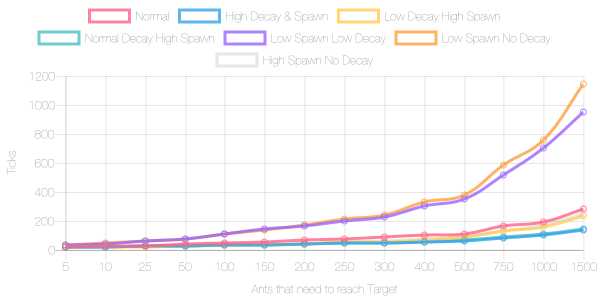
\includegraphics[width=1\linewidth]{images/mirroredwithtower-ticks-line}
  \caption{Comparing required Tick-Amount on the y-Axis to the target amount of ants to reach the target on the x-Axis for the mirrored map with normal settings}
  \label{fig:diffsettings}
\end{figure}

\begin{figure}[H]
  \centering
  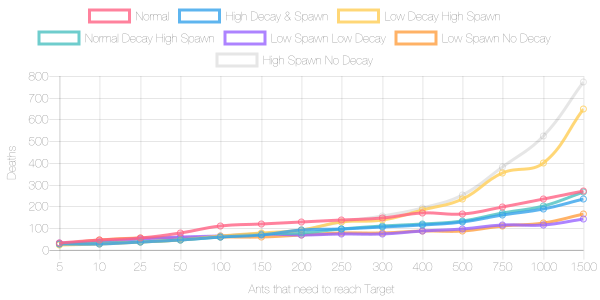
\includegraphics[width=1\linewidth]{images/mirroredwithtower-deaths-line}
  \caption{Comparing amount of deaths on the y-Axis to the target amount of ants to reach the target on the x-Axis for the mirrored map with normal settings}
  \label{fig:diffsettingsdeath}
\end{figure}

We have also already shown that the spawn-amount only has a logical impact on the tick amount and 14 is a good number given the damage of the towers. Now we also want to prove that the pheromone increase and decrease-level we declared as \textit{normal} are optimal
For that Figure \ref{fig:diffsettings2} compares the amount of ticks and Figure \ref{fig:diffsetting2sdeath} the amount of deaths for different pheromone-settings with the spawn amount 14 on the mirrored map.

As we can see the best value is in both instances achieved by the completely normal settings. It also shows that a low increase or also decay can negatively influence runtime. Also using a low pheromone increase can cause more deaths.

\begin{figure}[H]
  \centering
  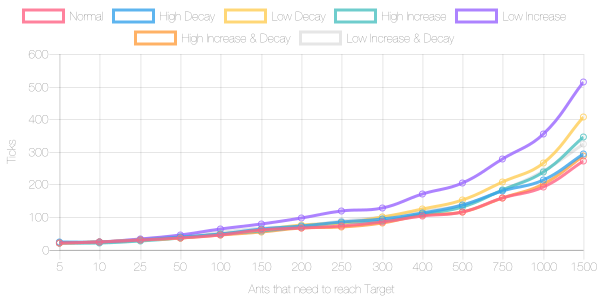
\includegraphics[width=1\linewidth]{images/mirrorednormalpheromticks}
  \caption{Comparing required Tick-Amount o n the y-Axis to the target amount of ants to reach the target on the x-Axis for the mirrored map with varying settings}
  \label{fig:diffsettings2}
\end{figure}

\begin{figure}[H]
  \centering
  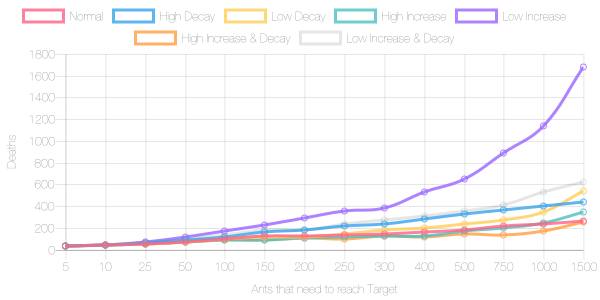
\includegraphics[width=1\linewidth]{images/mirroredwittowerdeaths}
  \caption{Comparing amount of deaths on the y-Axis to the target amount of ants to reach the target on the x-Axis for the mirrored map with normal settings}
  \label{fig:diffsetting2sdeath}
\end{figure}